% !TeX root = ../../Thesis.tex
\chapter{Effects of an External Magnetic Field on Stimulated Raman Scattering in homogeneous plasmas}
\label{chp:magSRS}

\section{Motivation and literature review}
\subsection{Magnetic suppression}
\subsection{Magnetic enhancement}
Suppress SRS to reduce harmful electrons and reflectivity, or enhance if it actually makes good electrons (in the case of shock-ignition).

\section{Magnetic field effect varies with plasma debye length}
\subsection{Rescatter}
\subsection{Kinetic inflation}
\subsection{Trapped particle modulation instability}

\section{Magnetic field effect changes with polarisation}

Start by replicating results from \cite{Winjum2018}

\begin{figure}
    \centering
    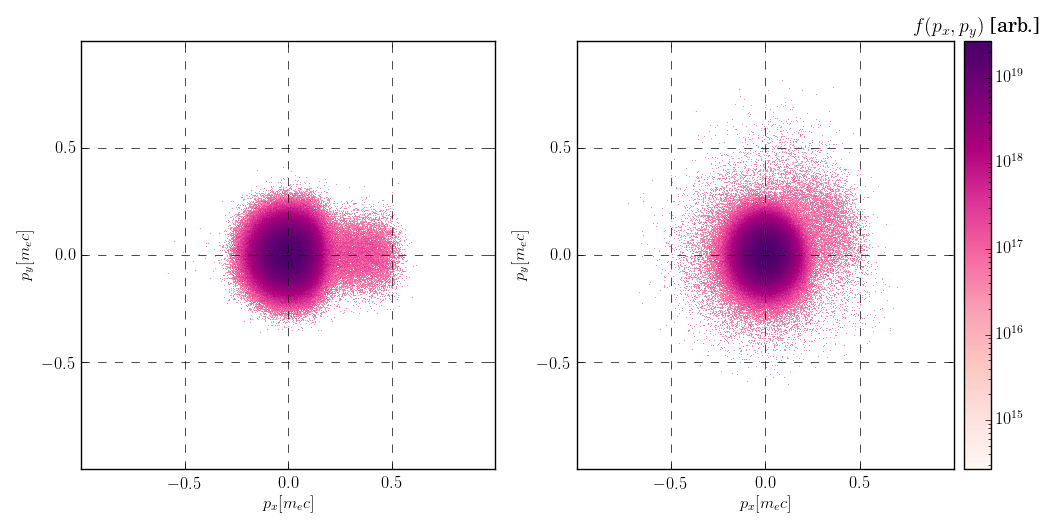
\includegraphics[width=0.99\textwidth]{Chapters/C6_magSRS/best_px_py_compare.png}
    \caption{Caption}
    \label{fig:my_label}
\end{figure}{}